% !TeX root = ../main.tex
% Add the above to each chapter to make compiling the PDF easier in some editors.

\chapter{Introduction}\label{chapter:introduction}
%Use with pdfLaTeX and Biber.
In this chapter, we will define key terms essential for understanding the thesis topic. We will discuss the architecture of AUTOSAR and the ECU along with its various software parts. Finally, we will connect these concepts to outline the primary objective of the thesis and highlight my key contributions.

\section{The AUTOSAR software architecture}
The AUTOSAR (Automotive Open System Architecture) standard defines an architecture for embedded software on ECUs \cite{autosar2022}. AUTOSAR systems can be divided in four main components (see ~\autoref{fig:AUTOSAR}):
\begin{figure}[htpb]
  \centering
  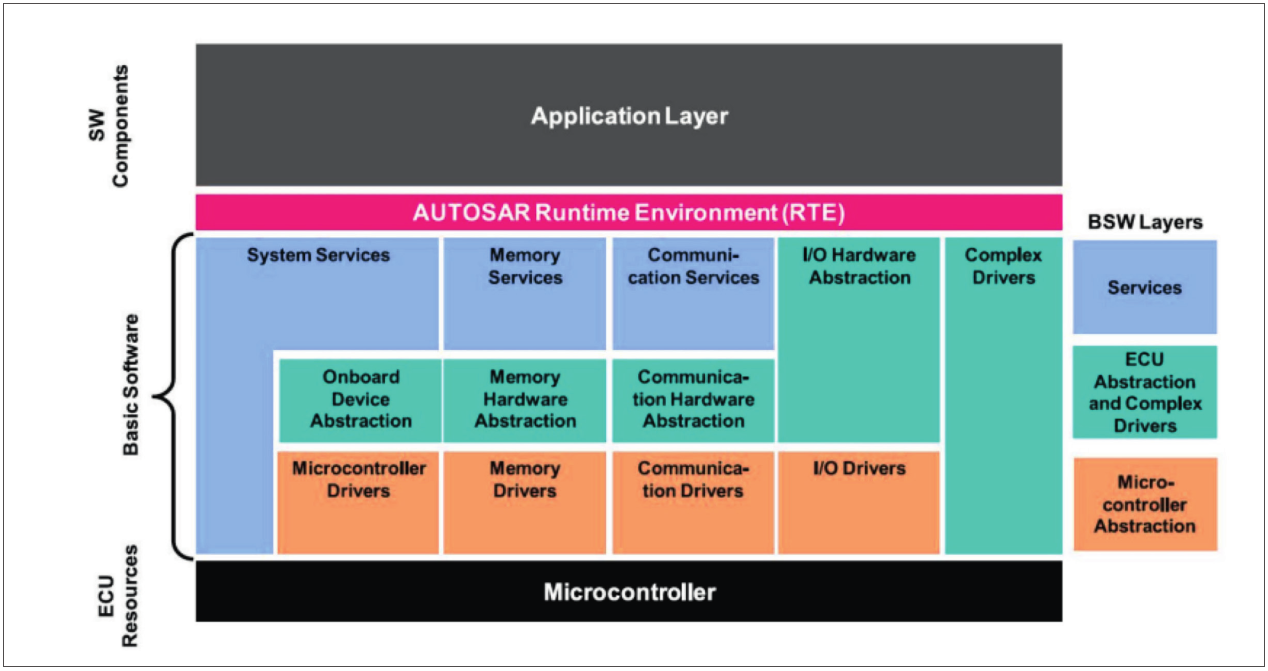
\includegraphics[width=1\textwidth]{figures/AUTOSAR}
  \caption{AUTOSAR (Classic Platform) ECU software layers \cite{smartse2020}.} \label{fig:AUTOSAR}
\end{figure}
\begin{enumerate}
\item \textbf{Application Software (ASW)} is the “highest layer” and comprises the control algorithm itself. This layer is called “Application Layer”. The content of this layer is, in most cases, the “system under test” (SUT). The BAC software components are located in this layer.
\item \textbf{Runtime Environment (RTE)} is the communication layer which distributes the signals directly between ASW components or using the base software’s (BSW) communication stack. The idea of AUTOSAR ASW components is that they can be distributed freely on different ECUs. The RTE will then either dispatch the data from one component directly to another component, if they are deployed on the same ECU, or the data is sent via the communication stack in the basic software.
\item \textbf{Basic Software (BSW)} is a software that provides a basic functionality of an ECU. The AUTOSAR Basic Software is further divided in the layers: Services, ECU Abstraction, Microcontroller Abstraction and Complex Drivers.
\begin{enumerate}
\item The Microcontroller Abstraction Layer (MCAL) is the lowest layer of the Basic Software. It manages access to the hardware, ensuring that high-level software does not directly interact with microcontroller registers. As a hardware-specific layer, MCAL provides a standardized interface for the basic software components, handling microcontroller peripherals and supplying them with hardware-independent values. MCAL also implements notification mechanisms to distribute commands, responses, and information across different processes. It can include components such as Digital I/O, Analog/Digital converters, Flash, and EEPROM.
\item The ECU Abstraction Layer interfaces the drivers of the Microcontroller Abstraction
Layer. It also contains drivers for external devices. It offers an API for access to peripherals and devices regardless of their location (µC internal/external) and their connection to the
µC (port pins, type of interface)
\item The Complex Drivers Layer spans from the hardware to the RTE, enabling direct access to Basic Software and/or hardware for resource-critical applications. It supports the integration of specialized functionality, such as drivers for devices not specified within AUTOSAR, those with strict timing constraints, or for migration purposes.
\item The Services Layer is the highest layer of the Basic Software. It provides essential functionalities, including operating system features, vehicle network communication and management services, memory services like NVRAM management, and diagnostic services such as UDS communication, error memory, and fault handling.
\end{enumerate}
\item \textbf{Microcontroller} is the actual hardware, which contains Internal devices, such as EEPROM, CAN controller, and ADC.
\end{enumerate}
\newpage
\begin{wrapfigure}{r}{0.4\textwidth}
  \centering
  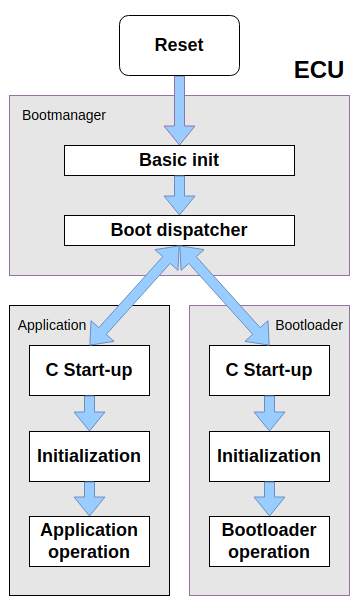
\includegraphics[width=0.9\linewidth]{figures/ECU.PNG}
  \caption{ECU Architecture.} \label{fig:ECU}
\end{wrapfigure}
\section{ECU Overall Architecture}\label{section:ECU_architecture}
Automotive ECUs typically contain three separate software parts, the Application, the bootmanager (BM), and the bootloader (BL).  After hardware or software reset of the ECU, the Bootmanager does certain basic initializations, and then jumps to the application or the bootloader. The bootmanager has no bus interface and no operating system. The Application implements the specific functionality of the ECU, e.g. controlling the engine or the airbags. The Bootloader allows to update the Application once the vehicle has been put on the market. ~\autoref{fig:ECU} provides an overview of the ECU overall architecture.

Although Application, Bootmanager and Bootloader are separate software parts, they require to exchange a minimum of information. This information is exchanged using a shared memory. After checking different conditions and flags, the bootmanager decides whether the Application or the Bootloader are started after a Reset. The Application is started, if there is no reprogramming request and the Application is valid. The Bootloader is started, if there is a reprogramming request or the Application is not valid. \cite{vectorBootloader} 

\section{Objective of the Thesis}
The main objective of this thesis is to develop a fully virtualized test environment tailored for the BMW AUTOSAR Core (BAC) software, enabling early software testing and more efficient debugging without relying on physical hardware. The virtualized environment is designed to replicate the functionality of a physical ECU using a virtual ECU and a virtual CAN bus. The goal is to enable ECU testing tools to interact with the vECU, send and receive CAN messages, and mimic the real ECU's behavior, including switching between various ECU modes.

\section{Thesis Contribution}
To create the virtual test setup, several missing components in the simulation needed to be developed. My primary contributions in this thesis include:
\begin{enumerate}
\item \textbf{Integrating the vECU into the test simulation}, enabling the testing of software components in a virtualized setup.
\item \textbf{Implementing an adapter} to facilitate communication between the vECU and the virtual CAN (vCAN) bus.
\item \textbf{Enabling data sharing between different ECU modes} to accurately represent real-world ECU behavior.
\item \textbf{Creating a unified simulation} that incorporates all ECU modes, allowing for accurate simulation of mode transitions, such as during resets or updates.
\item \textbf{Adjusting the timing} in the virtual environment to synchronize with real time, ensuring compatibility with testing tools that operate on a real-time basis, enabling accurate testing of the vECU.
\end{enumerate}

\section{Thesis Outline}
The structure of this thesis is organized as follows:
\begin{enumerate}
\item \textbf{Chapter 2} investigates state-of-the-art virtualization techniques and explores how similar projects use simulation, providing insight into different approaches.
\item \textbf{Chapter 3} compares traditional test setups with the virtual test setup implemented in this project. It introduces the software used in the virtual environment and the various testing tools employed.
\item \textbf{Chapter 4} details the core contributions of the thesis, focusing on the implementation of the adapter and the unified simulation. It provides an in-depth discussion of how these components were developed and integrated into the virtual environment.
\item \textbf{Chapter 5} discusses how virtual and real-time synchronization was achieved. It also presents the results of tests conducted on both the virtual and hardware setups, emphasizing the reliability of the virtual test environment in simulating real-world conditions.
\item The thesis concludes with a summary and a discussion of potential future work that could further enhance the virtual test environment.
\end{enumerate}